\documentclass[12pt]{article}
\usepackage{geometry}                % See geometry.pdf to learn the layout options. There are lots.
\geometry{a4paper,
 total={170mm,257mm},
 left=20mm,
 top=20mm,
 bottom=40mm}                   % ... or a4paper or a5paper or ... 
%\geometry{landscape}                % Activate for for rotated page geometry
\usepackage[parfill]{parskip}    % Activate to begin paragraphs with an empty line rather than an indent
\usepackage{graphicx}
\usepackage{amssymb}
\usepackage{epstopdf}
\usepackage{float}
\usepackage{hyperref}
\hypersetup{%
  colorlinks=true,% hyperlinks will be coloured
  linkcolor=blue,% hyperlink text will be green
}
\DeclareGraphicsRule{.tif}{png}{.png}{`convert #1 `dirname #1`/`basename #1 .tif`.png}
\graphicspath{ {/Users/olga/Desktop/TemplateRNAseq/!Documentation/Results/} }

%% LOGOS
\usepackage{fancyhdr}
%\setlength{\headheight}{1.5cm}
\addtolength{\headheight}{2cm} % make more space for the header
\pagestyle{fancyplain} % use fancy for all pages except chapter start
\lhead{
\includegraphics[height=1.3cm, width=2cm]{BILS-logo.pdf}} % left logo
\rhead{
\includegraphics[height=1.3cm, width=4cm]{SciLifeLab-logo.jpg}} % right logo
\renewcommand{\headrulewidth}{0pt} % remove rule below header

%% DEFINE TOOLS AND VARIABLES
\newcommand{\staff}{Olga Dethlefsen}
\newcommand{\staffWeb}{https://bils.se/staff/olga-dethlefsen/index.html}
\newcommand{\affilations}{Bioinformatics Infrastructure for Life Sciences, Science for Life Laboratory, Stockholm University}
\newcommand{\supportWeb}{https://bils.se/resources/support.html}
\newcommand{\uppmaxWeb}{http://www.uppmax.uu.se/faq/how-to-acknowledge-uppmax-snic-and-uppnex}
\newcommand{\noIssue}{\#9999}
\newcommand{\noUppmax}{b29999}
\newcommand{\fastqc}{\texttt{FastQC/0.11.2}}
\newcommand{\trimmomatic}{\texttt{trimmomatic/0.32}}
\renewcommand{\star}{\texttt{star/2.4.1c}}
\newcommand{\refGenome}{\texttt{Mus\_musculus.GRCm38.\-dna.primary\_assembly.fa}}
\newcommand{\refAnnotation}{\texttt{Mus\_musculus.GRCm38.81.gtf}}
\newcommand{\refSource}{\texttt{http://www.ensembl.org/index.html}}
\newcommand{\featureCounts}{\texttt{featureCounts/1.5.0}}
\newcommand{\subread}{\texttt{subread/1.4.5}}
\newcommand{\samtools}{\texttt{samtools/0.1.19}}
\newcommand{\multiqc}{\texttt{MultiQC/0.3.1}}
\newcommand{\homer}{\texttt{homer/4.7.2}}

%% BEGIN DOCUMENT
%\date{}
\usepackage{Sweave}
\begin{document}
\pagestyle{fancy}
\Sconcordance{concordance:9999_report.tex:9999_report.rnw:%
1 52 1 1 0 103 1 1 30 1 1 1 33 2 1 2 2 5 1 2 2 5 1 2 2 4 1 1 19 5 1 2 2 %
3 1 1 33 2 1 1 10 11 0 1 11 22 0 1 3 2 1 1 5 1 2 5 1 1 8 1 2 5 1 1 10 %
11 0 1 11 22 0 1 3 2 1 1 5 1 2 5 1 1 8 1 2 108 1 1 12 3 1 1 2 6 0 1 2 %
12 1 1 2 43 0 1 2 11 1}


%% TITLE PAGE
\title{Template for RNA-seq bioinformatics support}
\author{}
\maketitle
\thispagestyle{fancy}

\vspace{2cm}
\begin{center}
\begin{tabular}{l r}
Issue number: & {\noIssue} \\
Request by: & Jan User \\ 
Principal Investigator: & Maria Investigator \\
Organisation: & Stockholm University \\
BILS staff: & {\staff}
\end{tabular}
\end{center}

%% TABLE OF CONTENTS
\newpage
\tableofcontents

%% SUPPORT REQUEST
\newpage
\section{Support request}

To answer our question we have performed RNA-seq, total RNA ribosomal RNA depleted. We had 4 groups and would like help to finding differentially expressed genees


%% MATERIALS AND METHODS SECTION
\section{Materials and Methods}
\subsection{Available data}
Data were delivered to Inbox on Uppnex {\noUppmax} in fastq format using Illumina 1.8 quality scores. Data were from a paired-end run, with one file for the forward reads and one file for the reverse reads following a naming convention: [LANE\_[DATE]\_[FLOWCELL]\_[SCILIFE NAME]\_[READ].fastq.gz. 

\subsection{Data processing}
Raw sequencing reads were processed to obtain counts per genes for each samples. This included: 
\begin{enumerate}
  \item {\fastqc} quality check on raw sequencing reads
  \item {\trimmomatic} reads filtering for quality score and read length. Reads with average quality below 20 (within 4-base wide sliding window) and/or shorter than 36 bases were removed
  \item {\star} was used to align the reads to the reference genome {\refGenome} using the annotation {\refAnnotation}, with reference genome and annotation downloaded from {\refSource}
  \item {\featureCounts} from {\subread} was used to count the fragments in the exon regions as defined in the {\refAnnotation} file, using default parameters. Specifically, for paired-end reads, a fragment is said to overlap a feature if at least one read base is found to overlap the feature. Fragments overlapping with more than one feature and multi-mapping reads are not counted
  \item Counts from multiple lanes were added, if applicable
  \item {\samtools} were used to sort and index the BAM files containing the aligned reads, e.g. for visualisation in \href{https://www.broadinstitute.org/igv/}{IGV} genome browser 
  \item {\multiqc} was used to aggregate results from {\fastqc}, {\star} and {\featureCounts} across many samples into a single report
\end{enumerate}

\subsection{Differential expression}
All analyses were performed under \texttt{R}, a programming language and software environment for statistical computing and graphics. Details on the \texttt{R} version and packages used can found at the end of this document in \nameref{sessionInfo}
\begin{enumerate}
  \item \texttt{biomaRt} package was used to annotate Ensembl gene identifiers with chromosome name, official gene symbol and description. 
  \item low count reads were filtered by keeping reads with at least 1 read per million in at least 2 samples
  \item \texttt{edgeR} package was used to normalise for the RNA composition by finding a set of scaling factors for the library sizes that minimize the log-fold changes between the samples for most genes, using a trimmed mean of M values (TMM) between each pair of samples.
  \item the normalized counts were used to examine the samples for outliers and relationships, using Multidimensional Scaling and heatmap based on the Pearson correlation coefficient between every sample pair
    \item the normalized counts were used to examine the samples for outliers and relationships, using Multidimensional Scaling and heatmap based on the Pearson correlation coefficient between every sample pair
    \item \texttt{edgeR} package was to define design matrix based on the experimental design, fitting gene-wise glms model and conducting likelihood ratio tests for the selected group comparisons
\end{enumerate}

\subsection{Exon usage}
\begin{enumerate}
  \item \texttt{DEXseq} package in \texttt{R} was used to infer differential exon usage
  \item the provided with the \texttt{DEXseq} package \texttt{Python} scripts were used to prepare a flattened GTF file based on the {\refAnnotation} and to obtain counts per each exon given the aligned BAM files
  \item size factors measuring the relative sequencing depth were estimated to adjust for coverage biases
  \item variability of the data was then estimated to be able to distinguish technical and biological variation from real effects on exon usage due to the different conditions. Briefly, per-exon dispersions are calculated using a Cox-Reid adjusted profile likelihood estimation, then a dispersion-mean relation is fitted to this individual dispersion values and finally, the fitted values are taken as a prior in order to shrink the per-exon estimates towards the fitted values
  \item having the dispersion estimates and the size factors, differential exon usage was tested. For each gene, \texttt{DEXSeq} fits a generalized linear model with the formula \( \sim samples + exon + condition:exon\) and compares it to the null model  \( \sim samples + exon\). The deviances of both fits are compared using a $\chi^2$-distribution, giving rise to a p value, indicative wether the null model is sufficient to explain the data or whether it may be rejected in favour of the alternative containing an interaction coefficient for condition$\colon$exon. The latter means that the fraction of the gene's reads that fall onto the exon under the test differs significantly between the experimental conditions.
  \item the obtained p-values were BH adjusted for multiple comparison
\end{enumerate}

\subsection{HOMER Motif Analysis}
\begin{enumerate}
  \item {\homer} was used to analyze the promoters of genes and look for motifs that are enriched in the target gene promoters relative to other pomoters. The analyses followed the \href{http://homer.salk.edu/homer/motif/index.html}{'Analyzing lists of genes with promoter motif analysis' tutorial}
  \item briefly, for each comparison, the analyses were run for the differentially expressed genes, separately for down- and up-regulated genes, were differentially expressed genes were defined at 5\% FDR and absolute minimum log 2 fold change of 1. 
  \item the analyses included Gene Ontology enrichment calculations, \textit{de novo} motif analysis and known motif enrichment analysis
\end{enumerate}


%% WORK LOG SECTION
\section{Work log}
A brief project history containing key points
\begin{description}
\item[2015-09-15] first meeting with Jan to discuss experimental design, available data and desired results.	As first results, Jan would like to receive lists of differentially expressed (DE) genes between the two time points for the two groups
\item[2015-10-09] meeting with Jan to go over the DE results. Agreed that Jan will go over the DE results and try running gene set enrichment analyses using DAVID website.
\item[2015-11-06] I have run and emailed Jan the exon usage results for the 4 comparisons
\item[2015-12-01] I have run and emailed Jan the motif discovery Homer results
\item[2015-12-10] meeting with Jan to discuss the additional results
\end{description}

\section{Important practical information}
\subsection{Data responsibility}
Unfortunately, we do not have resources to keep any files associated with the support request. We kindly suggest that you store safely the results delivered by us. In addition, we kindly ask that you remove the files from UPPMAX/UPPNEX {\noUppmax}. The main storage at UPPNEX is optimized for high-speed and parallell access, which makes it expensive and not the right place for longer time archiving. Please consider others by not taking up the expensive space.
\subsection{Acknowledgments}
If you are presenting the results in a paper, at a workshop or conference, we kindly ask you to acknowledge us.
\begin{description}
\item[BILS staff] are encouraged to be co-authors when this is merited in accordance to the ethical recommendations for authorship, e.g. {\href{http://www.icmje.org/recommendations/}{ICMJE recommendations}}. If applicable, please include {\href{\staffWeb}{{\staff}, \affilations}} as co-author. In other cases, BILS would be grateful if support by us is acknowledged in publications according to this example: \href{https://bils.se/resources/support.html}{"Support by BILS (Bioinformatics Infrastructure for Life Sciences) is gratefully acknowledged."}
\item[Uppmax] kindly asks you to acknowledge UPPMAX and SNIC. If applicable, please add: {\href{\uppmaxWeb}{The computations were performed on resources provided by SNIC through Uppsala Multidisciplinary Center for Advanced Computational Science (UPPMAX) under Project {\noUppmax}.}}
\end{description}

\section{Results}
\subsection{Data exploration}
Table count, containing counts measured across many genes and samples, is a typical example of a multidimensional dataset, where \textit{N} objects (samples) were measured on \textit{p} numeric variables. Hence, to examine the samples for outliers and other relationship one can look at the several multivariate techniques that aim to reduce the dataset dimensions and to reveal the data structure by plotting samples in one or two dimensions. Multidimensional Scaling provides a visual representation of the pattern of proximities among a set of objects, here samples. Another method of visualisation is a heatmap based on the Pearson correlation coefficient, calculated between every sample pair. 

% INPUT

% BUILDING edgeR object, filtering and normalizing, preparing MDS frame

\begin{figure}[H]
\begin{center}
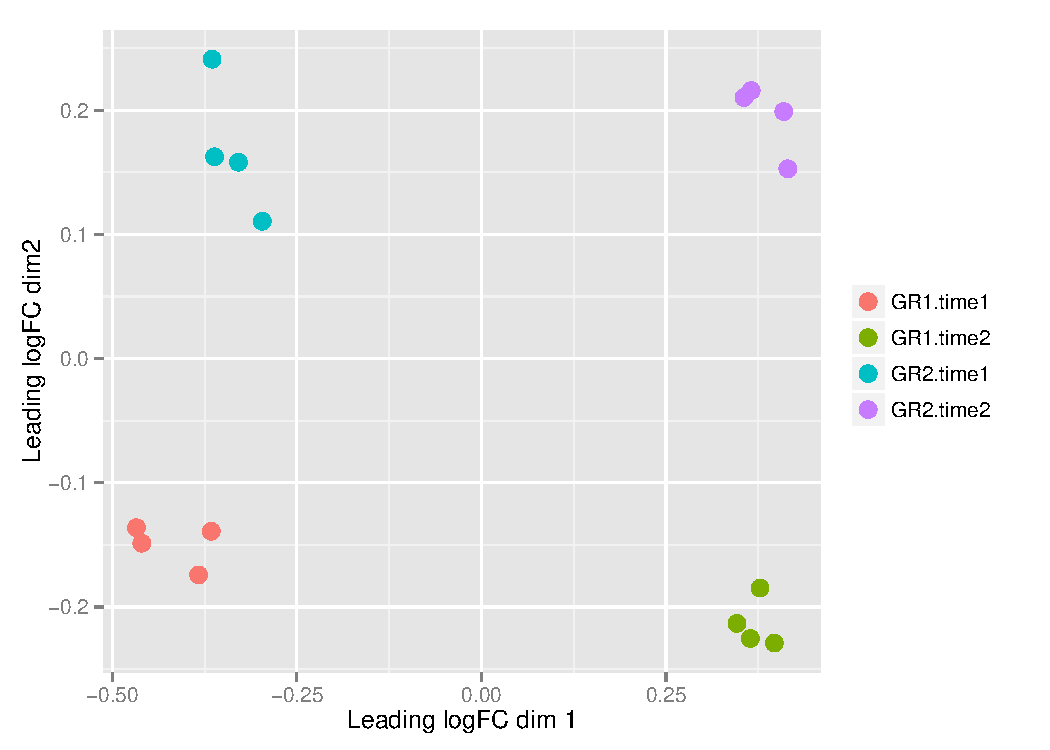
\includegraphics{9999_report-fig1}
\end{center}
\caption{MDS plot on the normalized and filtered counts colour-coded by samples groups}
\end{figure}  

\begin{figure}[H]
\begin{center}
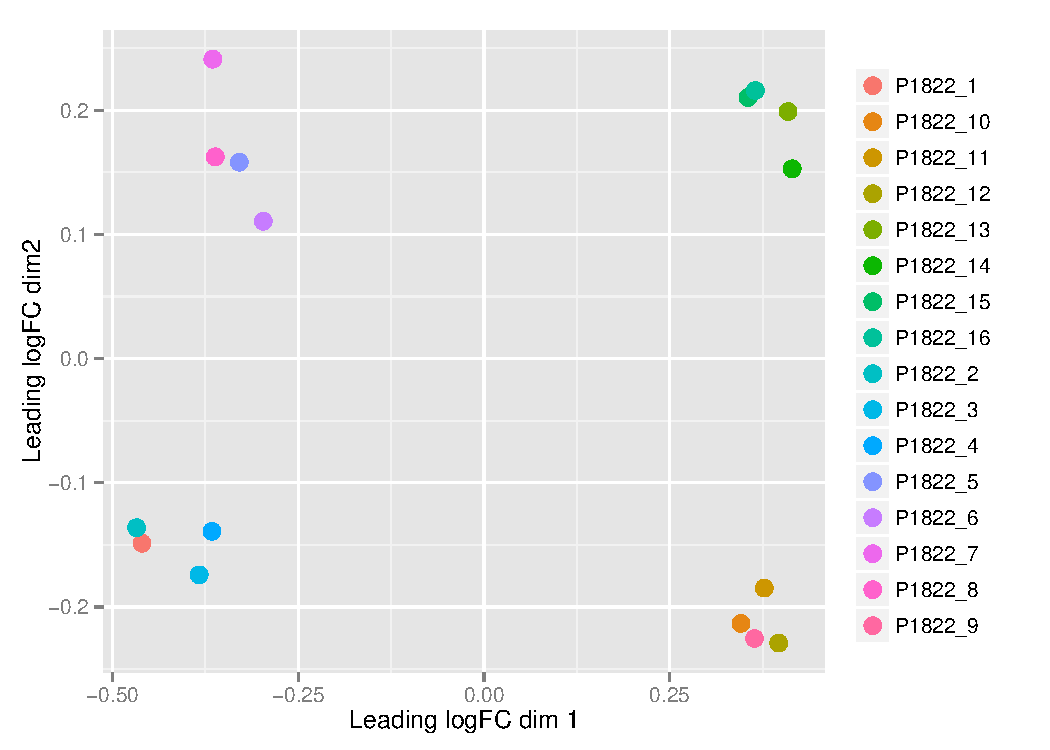
\includegraphics{9999_report-fig2}
\end{center}
\caption{MDS plot on the normalized and filtered counts colour-coded by individual samples}
\end{figure} 

\begin{figure}[H]
\begin{center}
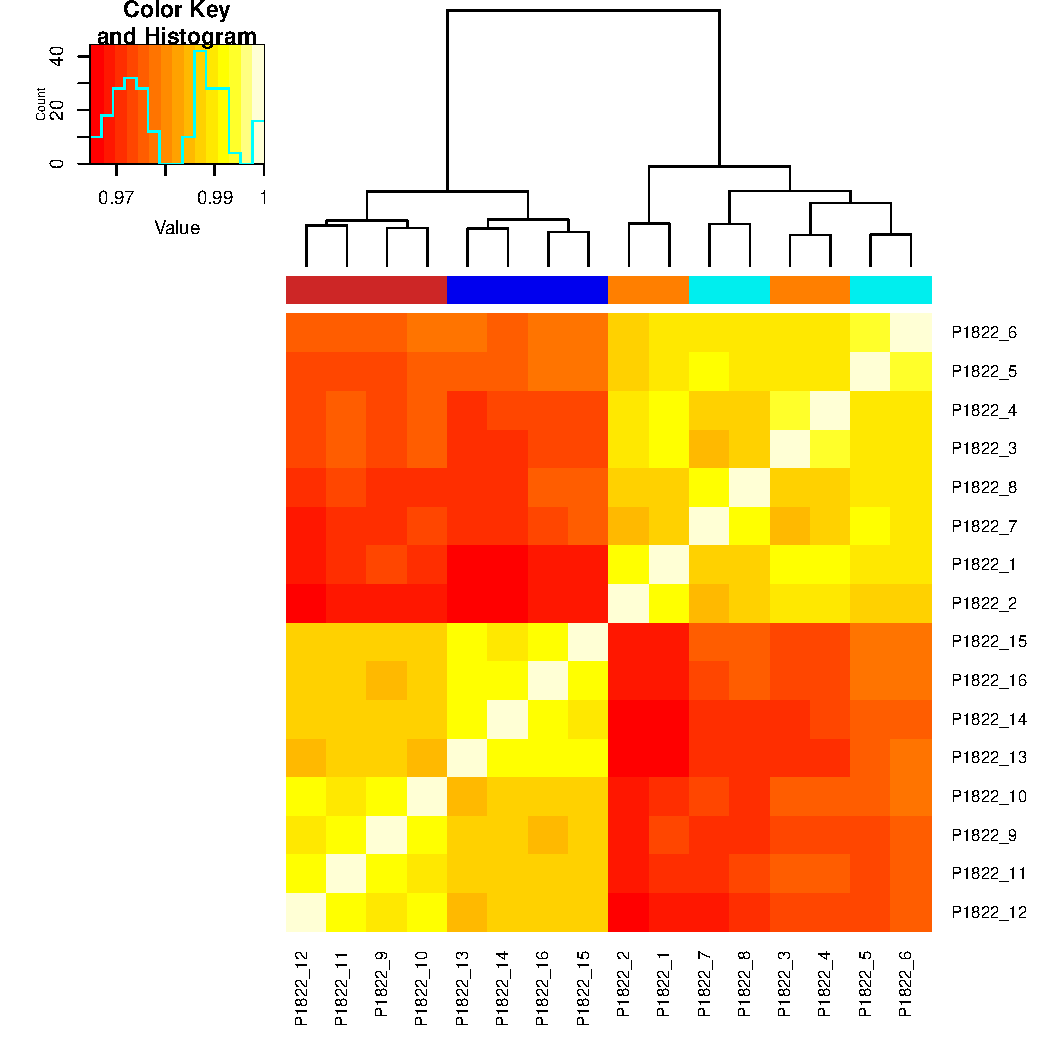
\includegraphics{9999_report-fig3}
\end{center}
\caption{Heatmap based on the pair-wise Pearson correlation coefficient between samples}
\end{figure} 

\subsection{Differential expression} 

\subsubsection{Estimating BCVs}
Two levels of variation, technical and biological, can be distinguished in any RNA-Seq experiment. Biological coefficient of variation (BCV) is the coefficient of variation with which the (unknown) true abundance of the gene varies between replicate RNA samples. It represents the CV that would remain between biological replicates if sequencing depth could be increased indefinitely. The technical CV decreases as the size of the counts increases. BCV on the other hand does not. BCV is therefore likely to be the dominant source of uncertainty for high-count genes, so reliable estimation of BCV is crucial for realistic assessment of differential expression in RNA-Seq experiments. \texttt{edgeR} uses empirical Bayes methods that permit the estimation of gene-specific biological variation, even for experiments with minimal levels of biological replication.

\begin{figure}[H]
\begin{center}
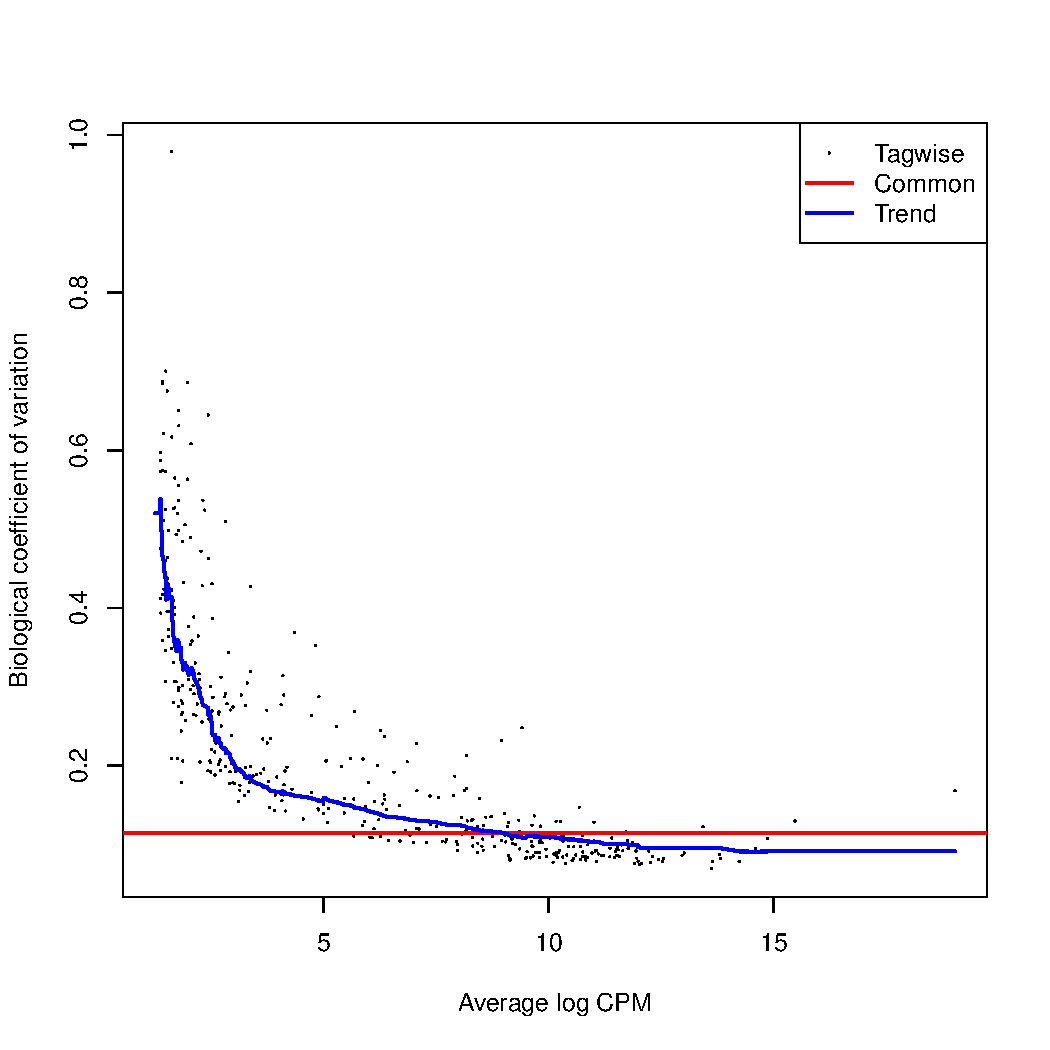
\includegraphics{9999_report-fig4}
\end{center}
\caption{Biological coefficient of variation plot showing the dispersion estimates}
\end{figure} 


\subsubsection{GR1: time2 vs. time1}

% latex table generated in R 3.2.2 by xtable 1.8-0 package
% Mon Feb 15 13:12:47 2016
\begin{table}[ht]
\centering
\begin{tabular}{rrrr}
  \hline
 & Down-regulated & Non-significant & Up-regulated \\ 
  \hline
Genes & 40 & 363 & 36 \\ 
   \hline
\end{tabular}
\caption{Number of down- and up-regulated differentially expressed genes given 5\% FDR and absolute minimum log-fold-change of 1 } 
\end{table}% latex table generated in R 3.2.2 by xtable 1.8-0 package
% Mon Feb 15 13:12:47 2016
\begin{table}[H]
\centering
{\footnotesize
\begin{tabular}{cccc}
  \hline
ensembl\_gene\_id & mgi\_symbol & GR1.logFC & GR1.FDR \\ 
  \hline
ENSMUSG00000056870 & Gulp1 & 2.33 & 3.33E-109 \\ 
  ENSMUSG00000025911 & Adhfe1 & 2.87 & 8.75E-82 \\ 
  ENSMUSG00000026064 & Ptp4a1 & -1.77 & 9.34E-75 \\ 
  ENSMUSG00000041859 & Mcm3 & -1.88 & 1.12E-63 \\ 
  ENSMUSG00000064294 & Aox3 & 4.29 & 4.36E-53 \\ 
  ENSMUSG00000026023 & Cdk15 & 3.67 & 6.06E-46 \\ 
  ENSMUSG00000038305 & Spats2l & -1.61 & 6.02E-44 \\ 
  ENSMUSG00000026069 & Il1rl1 & -1.63 & 4.74E-40 \\ 
  ENSMUSG00000026070 & Il18r1 & -2.63 & 3.72E-37 \\ 
  ENSMUSG00000051951 & Xkr4 & 3.28 & 1.31E-31 \\ 
   \hline
\end{tabular}
}
\caption{10 genes with the smallest FDR values} 
\end{table}
\begin{figure}[H]
\begin{center}
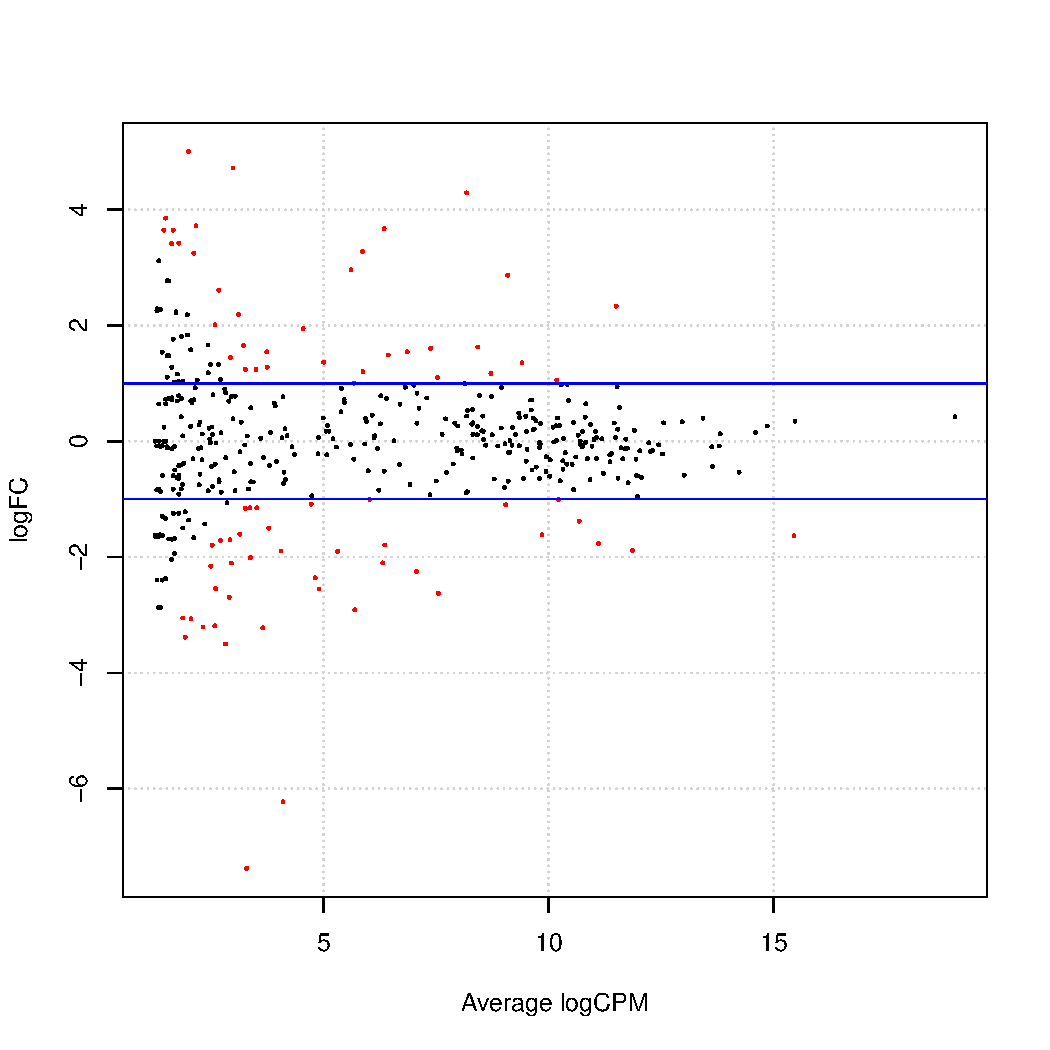
\includegraphics{9999_report-fig5}
\end{center}
\caption{Plot log-fold change against log-counts per million, with DE genes highlighted}
\end{figure} 

\begin{figure}[H]
\begin{center}
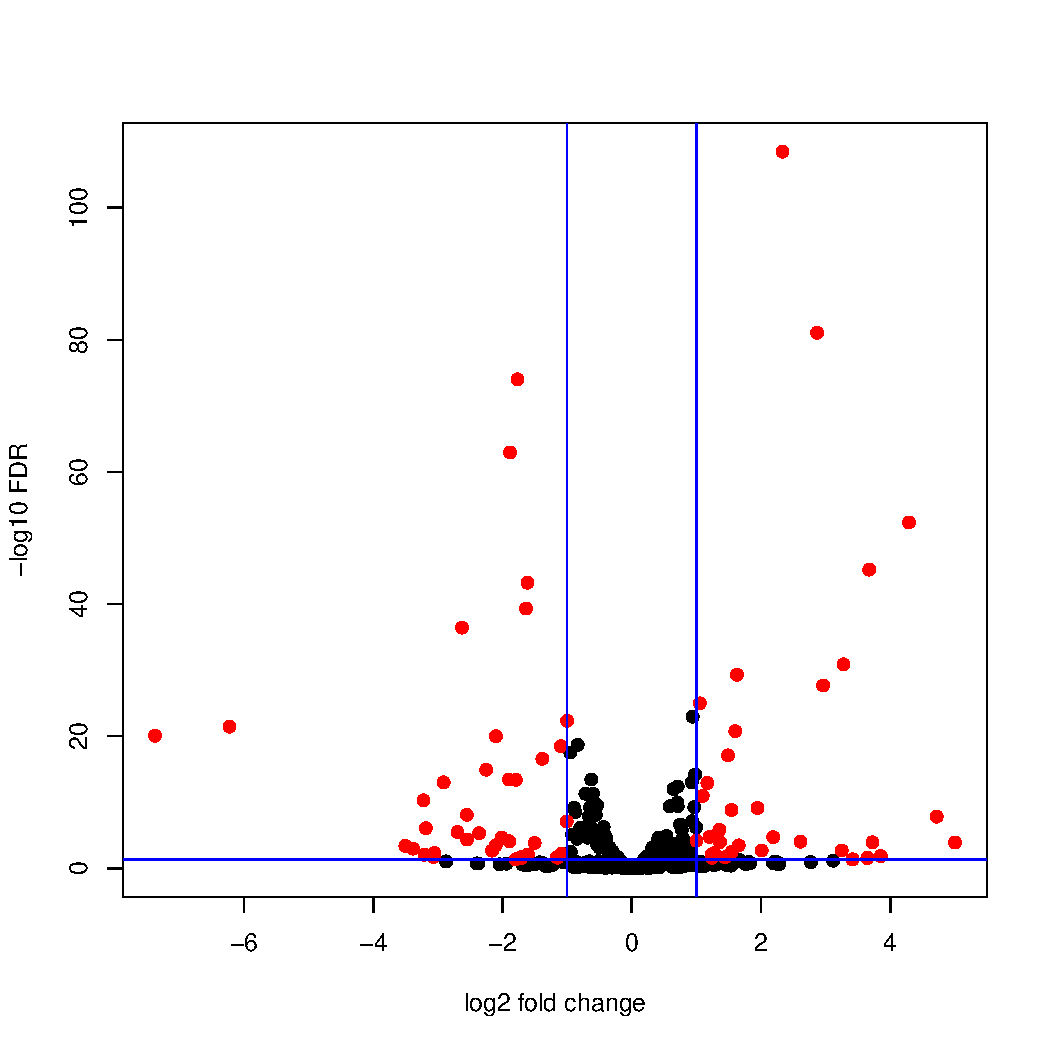
\includegraphics{9999_report-fig6}
\end{center}
\caption{Volcano plot with DE genes highlighted in red. Horizontal blue line corresponds to FDR=0.05 and vertical blue lines correspond to absolute log2 fold change of 1}
\end{figure} 

\subsubsection{GR2: time2 vs. time1}

% latex table generated in R 3.2.2 by xtable 1.8-0 package
% Mon Feb 15 13:12:47 2016
\begin{table}[ht]
\centering
\begin{tabular}{rrrr}
  \hline
 & Down-regulated & Non-significant & Up-regulated \\ 
  \hline
Genes & 36 & 368 & 35 \\ 
   \hline
\end{tabular}
\caption{Number of down- and up-regulated differentially expressed genes given 5\% FDR and absolute minimum log-fold-change of 1 } 
\end{table}% latex table generated in R 3.2.2 by xtable 1.8-0 package
% Mon Feb 15 13:12:47 2016
\begin{table}[H]
\centering
{\footnotesize
\begin{tabular}{cccc}
  \hline
ensembl\_gene\_id & mgi\_symbol & GR2.logFC & GR2.FDR \\ 
  \hline
ENSMUSG00000025993 & Slc40a1 & 3.20 & 3.50E-128 \\ 
  ENSMUSG00000056870 & Gulp1 & 2.34 & 3.02E-112 \\ 
  ENSMUSG00000026069 & Il1rl1 & -2.14 & 1.05E-65 \\ 
  ENSMUSG00000051951 & Xkr4 & 3.88 & 2.38E-58 \\ 
  ENSMUSG00000025911 & Adhfe1 & 2.31 & 4.00E-56 \\ 
  ENSMUSG00000026023 & Cdk15 & 4.07 & 5.65E-47 \\ 
  ENSMUSG00000064294 & Aox3 & 3.65 & 3.65E-43 \\ 
  ENSMUSG00000026070 & Il18r1 & -2.62 & 9.94E-39 \\ 
  ENSMUSG00000041859 & Mcm3 & -1.35 & 5.03E-34 \\ 
  ENSMUSG00000026064 & Ptp4a1 & -0.90 & 5.12E-20 \\ 
   \hline
\end{tabular}
}
\caption{10 genes with the smallest FDR values} 
\end{table}
\begin{figure}[H]
\begin{center}
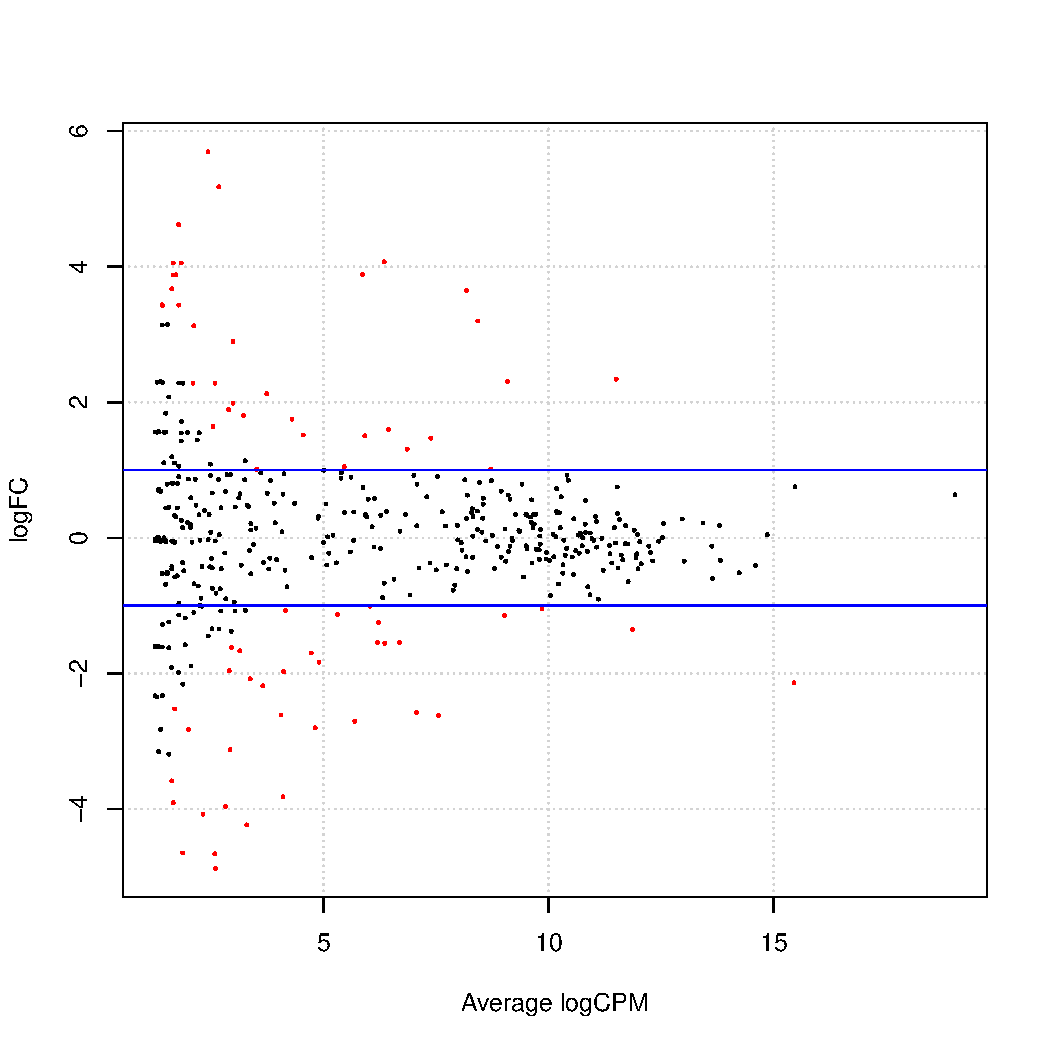
\includegraphics{9999_report-fig7}
\end{center}
\caption{Plot log-fold change against log-counts per million, with DE genes highlighted}
\end{figure} 

\begin{figure}[H]
\begin{center}
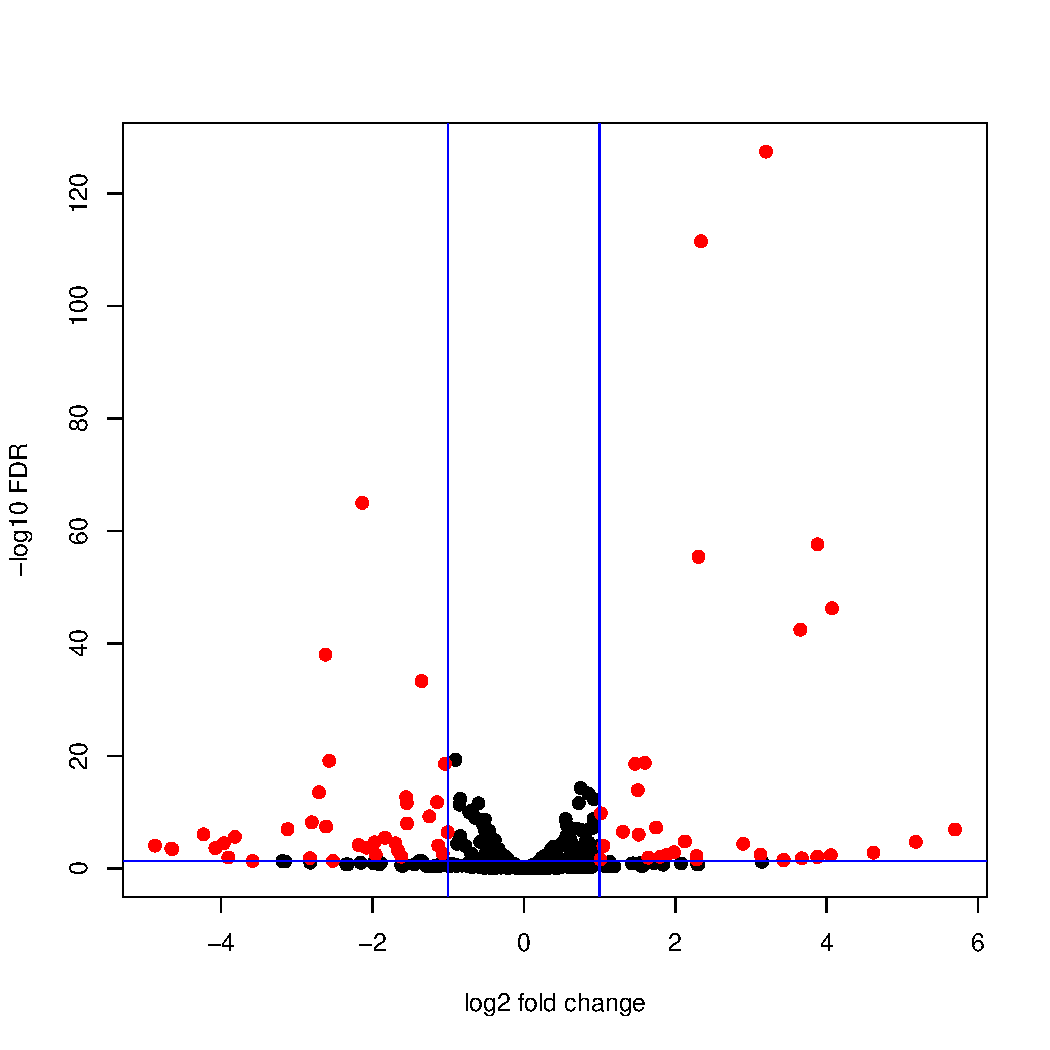
\includegraphics{9999_report-fig8}
\end{center}
\caption{Volcano plot with DE genes highlighted in red. Horizontal blue line corresponds to FDR=0.05 and vertical blue lines correspond to absolute log2 fold change of 1}
\end{figure} 

%' \subsubsection{NCS.48h vs. NCS.24h}
%' <<de3, echo=F, results=tex, include=F>>=
%' de3 <- function.de(data.cds$counts, table.annotations, fit, "NCS48vsNCS24")
%' tmp.de <- de3[[1]]
%' tmp.summary <- de3[[2]]
%' tmp.lrt <- de3[[3]]
%' 
%' # Number of down- and up-regulated
%' print(xtable(tmp.summary, digits=0,
%'       caption = "Number of down- and up-regulated differentially expressed genes given 5\\% FDR and absolute minimum log-fold-change of 1 "),
%'       caption.placement = "bottom")
%' 
%' # Top 10 changes
%' o <- order(tmp.de[,10])
%' table.out <- tmp.de[o[1:10],c(-2,-3,-5,-7,-8,-9)]
%' print(xtable(table.out, align=c("c","c","c","c","c"), display=c("s","s","s","f","E"),
%'       caption = "10 genes with the smallest FDR values"),
%'       caption.placement = "bottom",
%'       size="footnotesize",
%'       include.rownames=FALSE,
%'       floating=TRUE,
%'       table.placement="H")
%' 
%' @
%' 
%' \begin{figure}[H]
%' \begin{center}
%' <<label=fig9, fig=TRUE, echo=FALSE, width=7, height=7>>=
%'   de <- decideTestsDGE(tmp.lrt, lfc=1)
%'   detags <- rownames(data.cds)[as.logical(de)]
%'   plotSmear(tmp.lrt, de.tags=detags)
%'   abline(h=c(-1, 1), col="blue")
%' @
%' \end{center}
%' \caption{Plot log-fold change against log-counts per million, with DE genes highlighted}
%' \end{figure} 
%' 
%' \begin{figure}[H]
%' \begin{center}
%' <<label=fig10, fig=TRUE, echo=FALSE, width=7, height=7>>=
%'   lrt.top <- topTags(tmp.lrt, n=Inf, adjust.method='BH')
%'   lrt.table <- lrt.top$table  
%'   idx.sign <- match(detags, rownames(lrt.table))
%'   plot(lrt.table$logFC, -log10(lrt.table$FDR), pch=19, xlab='log2 fold change', ylab="-log10 FDR")
%'   points(lrt.table$logFC[idx.sign], -log10(lrt.table$FDR)[idx.sign], pch=19, col="red")
%'   abline(v=c(-1, 1), col="blue")
%'   abline(h=-log10(0.05), col="blue")
%' @
%' \end{center}
%' \caption{Volcano plot with DE genes highlighted in red. Horizontal blue line corresponds to FDR=0.05 and vertical blue lines correspond to absolute log2 fold change of 1}
%' \end{figure} 
%' 
%' \subsubsection{FBS.48h vs. FBS.24h}
%' <<de4, echo=F, results=tex, include=F>>=
%' de4 <- function.de(data.cds$counts, table.annotations, fit, "FBS48vsFBS24")
%' tmp.de <- de4[[1]]
%' tmp.summary <- de4[[2]]
%' tmp.lrt <- de4[[3]]
%' 
%' # Number of down- and up-regulated
%' print(xtable(tmp.summary, digits=0,
%'       caption = "Number of down- and up-regulated differentially expressed genes given 5\\% FDR and absolute minimum log-fold-change of 1 "),
%'       caption.placement = "bottom")
%' 
%' # Top 10 changes
%' o <- order(tmp.de[,10])
%' table.out <- tmp.de[o[1:10],c(-2,-3,-5,-7,-8,-9)]
%' print(xtable(table.out, align=c("c","c","c","c","c"), display=c("s","s","s","f","E"),
%'       caption = "10 genes with the smallest FDR values"),
%'       caption.placement = "bottom",
%'       size="footnotesize",
%'       include.rownames=FALSE,
%'       floating=TRUE,
%'       table.placement="H")
%' 
%' @
%' 
%' \begin{figure}[H]
%' \begin{center}
%' <<label=fig11, fig=TRUE, echo=FALSE, width=7, height=7>>=
%'   de <- decideTestsDGE(tmp.lrt, lfc=1)
%'   detags <- rownames(data.cds)[as.logical(de)]
%'   plotSmear(tmp.lrt, de.tags=detags)
%'   abline(h=c(-1, 1), col="blue")
%' @
%' \end{center}
%' \caption{Plot log-fold change against log-counts per million, with DE genes highlighted}
%' \end{figure} 
%' 
%' \begin{figure}[H]
%' \begin{center}
%' <<label=fig12, fig=TRUE, echo=FALSE, width=7, height=7>>=
%'   lrt.top <- topTags(tmp.lrt, n=Inf, adjust.method='BH')
%'   lrt.table <- lrt.top$table  
%'   idx.sign <- match(detags, rownames(lrt.table))
%'   plot(lrt.table$logFC, -log10(lrt.table$FDR), pch=19, xlab='log2 fold change', ylab="-log10 FDR")
%'   points(lrt.table$logFC[idx.sign], -log10(lrt.table$FDR)[idx.sign], pch=19, col="red")
%'   abline(v=c(-1, 1), col="blue")
%'   abline(h=-log10(0.05), col="blue")
%' @
%' \end{center}
%' \caption{Volcano plot with DE genes highlighted in red. Horizontal blue line corresponds to FDR=0.05 and vertical blue lines correspond to absolute log2 fold change of 1}
%' \end{figure} 

% Putting DE results together and saving files

%% WHAT HAS BEEN DELIVERED
\section{Deliverables}
Below is the list of key tab-delimited text files containing the key results from the described data analyses
\begin{Schunk}
\begin{Soutput}
[1] "DE.txt"                      "count_table.txt"            
[3] "count_table_annotations.txt" "norm_table.txt"             
[5] "norm_table_annotations.txt" 
\end{Soutput}
\end{Schunk}
where, 

\begin{description}
  \item[DE.txt] contains the differential expression results for all the analyses
  \item[count\_table.txt] contains the raw genes counts
  \item[count\_table\_annotations.txt] contains the annotations for the genes in the count\_table.txt
  \item[norm\_table.txt] contains filtered and normalized genes expression values (TMM)
  \item[norm\_table\_annotations.txt] contains the annotations for the norm\_table.txt
\end{description}

\section{R session info}
\label{sessionInfo}
%' and the number of samples is
\begin{Schunk}
\begin{Soutput}
R version 3.2.2 (2015-08-14)
Platform: x86_64-apple-darwin13.4.0 (64-bit)
Running under: OS X 10.10.5 (Yosemite)

locale:
[1] C

attached base packages:
[1] stats4    parallel  stats     graphics  grDevices utils     datasets 
[8] methods   base     

other attached packages:
 [1] DEXSeq_1.14.2             DESeq2_1.8.2             
 [3] RcppArmadillo_0.6.200.2.0 Rcpp_0.12.2              
 [5] GenomicRanges_1.20.8      GenomeInfoDb_1.4.3       
 [7] IRanges_2.2.9             S4Vectors_0.6.6          
 [9] Biobase_2.28.0            BiocGenerics_0.14.0      
[11] BiocParallel_1.2.22       xtable_1.8-0             
[13] biomaRt_2.24.1            gplots_2.17.0            
[15] ggplot2_1.0.1             edgeR_3.10.5             
[17] limma_3.24.15            

loaded via a namespace (and not attached):
 [1] genefilter_1.50.0    statmod_1.4.22       gtools_3.5.0        
 [4] locfit_1.5-9.1       reshape2_1.4.1       splines_3.2.2       
 [7] lattice_0.20-33      colorspace_1.2-6     XML_3.98-1.3        
[10] survival_2.38-3      foreign_0.8-66       DBI_0.3.1           
[13] RColorBrewer_1.1-2   lambda.r_1.1.7       plyr_1.8.3          
[16] zlibbioc_1.14.0      stringr_1.0.0        Biostrings_2.36.4   
[19] munsell_0.4.2        gtable_0.1.2         futile.logger_1.4.1 
[22] hwriter_1.3.2        caTools_1.17.1       labeling_0.3        
[25] latticeExtra_0.6-26  geneplotter_1.46.0   AnnotationDbi_1.30.1
[28] proto_0.3-10         acepack_1.3-3.3      KernSmooth_2.23-15  
[31] scales_0.3.0         gdata_2.17.0         Hmisc_3.17-0        
[34] annotate_1.46.1      XVector_0.8.0        Rsamtools_1.20.5    
[37] gridExtra_2.0.0      digest_0.6.8         stringi_1.0-1       
[40] grid_3.2.2           tools_3.2.2          bitops_1.0-6        
[43] magrittr_1.5         RCurl_1.95-4.7       RSQLite_1.0.0       
[46] Formula_1.2-1        cluster_2.0.3        futile.options_1.0.0
[49] MASS_7.3-45          rpart_4.1-10         nnet_7.3-11         
\end{Soutput}
\end{Schunk}

\section{Where to go next}
There is a wide selection of online user-friendly tools available for investigating the interesting genes or list of DE genes. Few recommended below 
\begin{description}
  \item[\href{hhttp://biit.cs.ut.ee/clustvis/}{ClustVist}] for creating Principal Component Analysis plots and heatmaps
  \item[\href{http://bioinfogp.cnb.csic.es/tools/venny/}{Venny}] helps to prepare Venn diagram showing relations between a finite collection of different sets, e.g. between list of DE genes from different comparisons
  \item[\href{https://david.ncifcrf.gov}{DAVID}] for a comprehensive set of functional annotation tools for investigators to understand biological meaning behind large list of genes, including identification of enriched Gene Ontology terms, discovering enriched functional-related gene groups, visualizing genes on BioCarta \& KEGG pathway and many more
  \item[\href{http://revigo.irb.hr}{REVIGO}] for summarizing long list of Gene Ontology terms and visualisation in semantic similarity-based scatterplots, interactive graphs or tag clouds
  \item[\href{http://funcoup.sbc.su.se/}{FunCoup}] for inferring genome-wide functional couplings or associations, that is an unspecific form of association that encompasses direct physical interaction but also more general types of direct or indirect interaction like regulatory interaction or participation the same process or pathway.
\end{description}

\end{document}  
